%15 min preso!
\documentclass[xcolor=table,aspectratio=169]{beamer}
\usepackage{beamerthemesplit}
\usepackage{wrapfig}
\usetheme{SPbGU}
\usepackage{pdfpages}
\usepackage{amsmath}
\usepackage{cmap}
\usepackage[T2A]{fontenc}
\usepackage[utf8]{inputenc}
\usepackage[english]{babel}
\usepackage{indentfirst}
\usepackage{amsmath}
\usepackage{tikz}
\usepackage{multirow}
\usepackage[noend]{algpseudocode}
\usepackage{algorithm}
\usepackage{algorithmicx}
\usepackage{fancyvrb}
\usepackage{hyperref} 
\usetikzlibrary{calc}
\usetikzlibrary{shapes, backgrounds}
\usetikzlibrary{arrows,automata}
\usetikzlibrary{positioning}
\usetikzlibrary{fit}
\usetikzlibrary{shapes.callouts}
\usetikzlibrary{shapes.misc}
\usepackage{xparse}
\usepackage{fontawesome}

\usepackage{etoolbox,refcount}
\usepackage{multicol}

\usepackage{tabularx}
\newcolumntype{Y}{>{\raggedleft\arraybackslash}X}

\renewcommand{\thealgorithm}{}

\newtheorem{mytheorem}{Theorem}
\renewcommand{\thealgorithm}{}

\newcommand{\tikzmark}[1]{\tikz[overlay,remember picture] \node (#1) {};}
\def\Put(#1,#2)#3{\leavevmode\makebox(0,0){\put(#1,#2){#3}}}

\newcommand{\ltz}{$< 1$}

\tikzset{
    state/.style={
           rectangle,
           rounded corners,
           draw=black, very thick,
           minimum height=2em,
           inner sep=2pt,
           text centered,
           },
}

\tikzset{
    invisible/.style={opacity=0,text opacity=0},
    visible on/.style={alt=#1{}{invisible}},
    alt/.code args={<#1>#2#3}{%
      \alt<#1>{\pgfkeysalso{#2}}{\pgfkeysalso{#3}} % \pgfkeysalso doesn't change the path
    },
}

\tikzset{cross/.style={cross out, draw=black, minimum size=2*(#1-\pgflinewidth), inner sep=0pt, outer sep=0pt, ultra thick},
%default radius will be 1pt. 
cross/.default={1pt}}

\NewDocumentCommand{\mycallout}{r<> O{opacity=0.8,text opacity=1} m m m}{%
\tikz[remember picture, overlay]\node[align=center, fill=cyan!20, text width=#5cm,
#2,visible on=<#1>, rounded corners,
draw,rectangle callout,anchor=pointer,callout relative pointer={(290:0.5cm)}]
at (#3) {#4};
}

\NewDocumentCommand{\mycalloutR}{r<> O{opacity=0.8,text opacity=1} m m m}{%
\tikz[remember picture, overlay]\node[align=center, fill=cyan!20, text width=#5cm,
#2,visible on=<#1>, rounded corners,
draw,rectangle callout,anchor=pointer,callout relative pointer={(30:0.8cm)}]
at (#3) {#4};
}


%callout relative pointer={(230:0.5cm)}]

\newcounter{countitems}
\newcounter{nextitemizecount}
\newcommand{\setupcountitems}{%
  \stepcounter{nextitemizecount}%
  \setcounter{countitems}{0}%
  \preto\item{\stepcounter{countitems}}%
}
\makeatletter
\newcommand{\computecountitems}{%
  \edef\@currentlabel{\number\c@countitems}%
  \label{countitems@\number\numexpr\value{nextitemizecount}-1\relax}%
}
\newcommand{\nextitemizecount}{%
  \getrefnumber{countitems@\number\c@nextitemizecount}%
}
\newcommand{\previtemizecount}{%
  \getrefnumber{countitems@\number\numexpr\value{nextitemizecount}-1\relax}%
}
\makeatother    
\newenvironment{AutoMultiColItemize}{%
\ifnumcomp{\nextitemizecount}{>}{3}{\begin{multicols}{2}}{}%
\setupcountitems\begin{itemize}}%
{\end{itemize}%
\unskip\computecountitems\ifnumcomp{\previtemizecount}{>}{3}{\end{multicols}}{}}


\beamertemplatenavigationsymbolsempty

\title[FLDDA Research Group Report]{Formal Language Driven Data Analysis Research Group Report}
\institute[SPbSU]{
Saint Petersburg State University
}

% То, что в квадратных скобках, отображается в левом нижнем углу.
\author[Semyon Grigorev]{Semyon Grigorev}

\date{April 26, 2023}


%Я предлагаю сначала в общем рассказать интересы и компетенции группы, 
%что научная группа сделала за 3 месяца, 
%потом потратить 1 страницу презентации на каждого из студентов (что сделал, почему важно для Yiming, какие планы). 
%В конце перейти к планам на год.

\begin{document}
{
\begin{frame}[fragile]
  \begin{table}
  \centering
  %
\includegraphics[height=1.5cm]{pictures/SPbGU_Logo.png}
  \begin{tabularx}{\linewidth}{XcX}
    
\includegraphics[height=0.9cm]{pictures/hu_logo.jpeg} \hfill
    & 
    & \hfill 
\includegraphics[height=1.6cm]{pictures/SPbGU_Logo.png}
  \end{tabularx}
  \end{table}
  \titlepage
\end{frame}
}

\begin{frame}[fragile]
  \frametitle{Research Landscape}  
  \begin{center}
    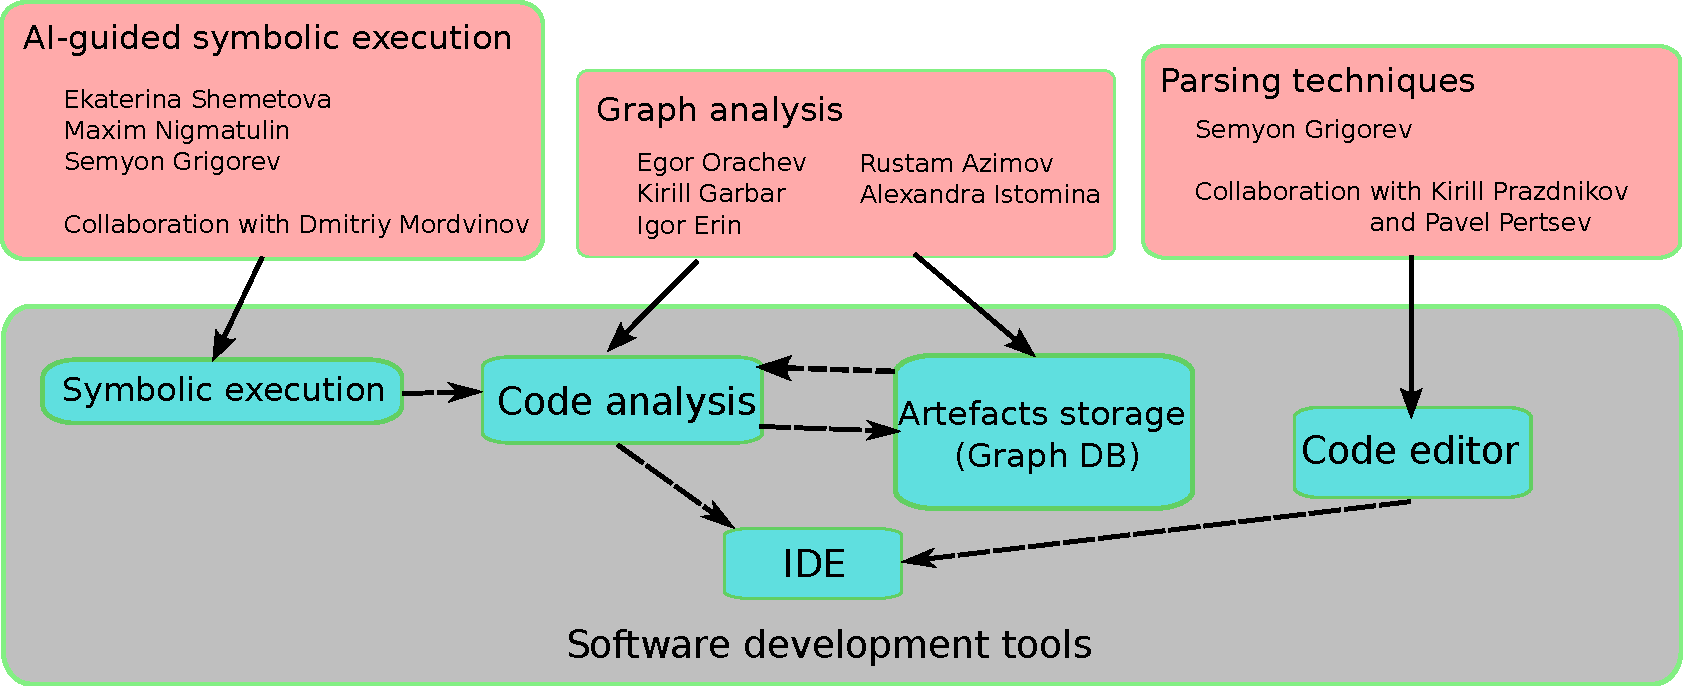
\includegraphics[width=\textwidth]{pictures/landscape.pdf}
  \end{center} 
\end{frame}


\begin{frame}[fragile]
  \frametitle{AI-Guided Symbolic Execution}  
  
  \begin{itemize}
    \item[\faCheck] Basic infrastructure for training developed and implemented
      \begin{itemize}
        \item Wrapper for SVM to convert it to server
        \item Python client --- AI agent to training
        \item Basic manipulation with neural networks 
      \end{itemize}
    \item[\faCheck] Basic dataset for train and validation/test
    \item[\faCheck] First attempts to train AI agent: workflow works fine (but agent too stupid to learn) 
    \item[\faGears] Dataset extension
    \item[\faGears] GNN improvement and pretraining 
    \item[\faGears] Performance tuning 
    \item[\faHourglassHalf] First version of AI agent which guide SVM on par with algorithmic strategies
  \end{itemize}
\end{frame}


\begin{frame}[fragile]
  \frametitle{Parsing Techniques}  
  
  \begin{itemize}
    \item[\faCheck] Partial parsing to improve highlighting speed for huge files
    \begin{table}[]
      \begin{tabular}{|l|l|llll|}
      \hline
      \multirow{3}{*}{File} & \multirow{3}{*}{Size} & \multicolumn{4}{l|}{Parsing time (ms)}                                                          \\ \cline{3-6} 
                            &                       & \multicolumn{2}{l|}{Web}                                  & \multicolumn{2}{l|}{Desktop}        \\ \cline{3-6} 
                            &                       & \multicolumn{1}{l|}{Partial} & \multicolumn{1}{l|}{Full}  & \multicolumn{1}{l|}{Partial} & Full \\ \hline \hline
      EUC\_TU\_OLD.java     & 2302Kb                & \multicolumn{1}{l|}{1386}    & \multicolumn{1}{l|}{11802} & \multicolumn{1}{l|}{417}     & 2271 \\ \hline
      \rowcolor[HTML]{FD6864}
      JavaParser.java       & 428Kb                 & \multicolumn{1}{l|}{666}     & \multicolumn{1}{l|}{6225}  & \multicolumn{1}{l|}{86}      & 1175 \\ \hline
      TestBigObj.java       & 1539Kb                & \multicolumn{1}{l|}{2324}    & \multicolumn{1}{l|}{3256}  & \multicolumn{1}{l|}{356}     & 664  \\ \hline
      INDIFY\_Test.Java     & 927Kb                 & \multicolumn{1}{l|}{1162}    & \multicolumn{1}{l|}{7756}  & \multicolumn{1}{l|}{206}     & 1925 \\ \hline
      \end{tabular}
      \end{table}
    \pause  
    \item[\faGears] Na\"{\i}ve incremental parsing 
    \item[\faGears] Error recovery mechanism
    \item[\faHourglassHalf] Advanced incremental parsing
  \end{itemize}
\end{frame}

\begin{frame}[fragile]
  \frametitle{Graph Analysis}  
  
  \begin{itemize}
    \item[\faCheck] Datalog-based static code analysis prototype implemented
    \item[\faGears] Datalog-based static code analysis evaluation
    \pause 
    \item[\faCheck] Spla --- vendor-agnostic sparse linear algebra for graph analysis on GPGPU
    \begin{itemize}
      \item OpenCL for GPU
      \item Intel, AND, Nvidia GPGs evaluated
    \end{itemize}
    \begin{center}
      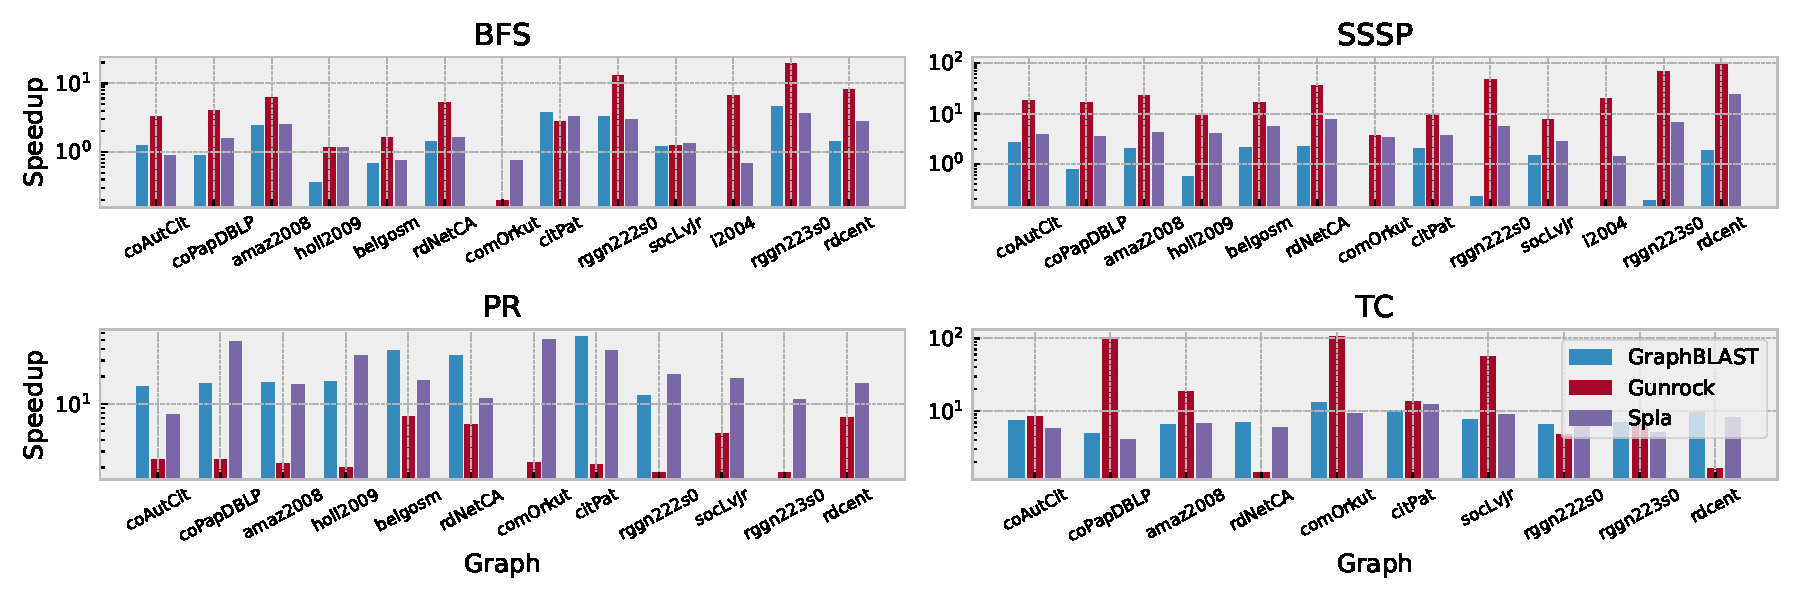
\includegraphics[width=0.9\textwidth]{pictures/rq1_rel.pdf}
    \end{center}
     
    \item[\faHourglassHalf] Performance tuning, more algorithms, \ldots
  \end{itemize}
\end{frame}

%\begin{frame}[fragile]
%  \frametitle{New Members (from June)}  
%  
%  \begin{itemize}
%      \item One in AI-based symbolic execution 
%      \item One in graph analysis
%  \end{itemize}
%\end{frame}


\end{document}
